\chapter{Introduction}

\textit{In this first chapter we want to familiarize the reader with the
scientific background of our work and its motivation. We hope to clarify what
basic questions the discipline of ultracold atom experiments tries to solve.
In a second part we want to elaborate on the concepts of localized optical
potential dynamics and summarize related work reported by the community.}

Many-body quantum systems studied inter alia in condensed matter physics are
experimentally challenging to access and investigate directly. As a way
forward, experiments with ultracold atoms in optical lattices give us a highly
controllable environment where you can access observables at a single atom
level, prepare clean, well-known quantum states and increase length and time
scales to experimentally accessible quantities. Thus the platform of ultracold
atoms in optical lattices permits us to simulate and explore quantum effects
and expand our current understanding of quantum mechanics and statistical
physics~\cite{Bloch2008,Gross2017}.
\begin{figure}[htb]
  \centering
  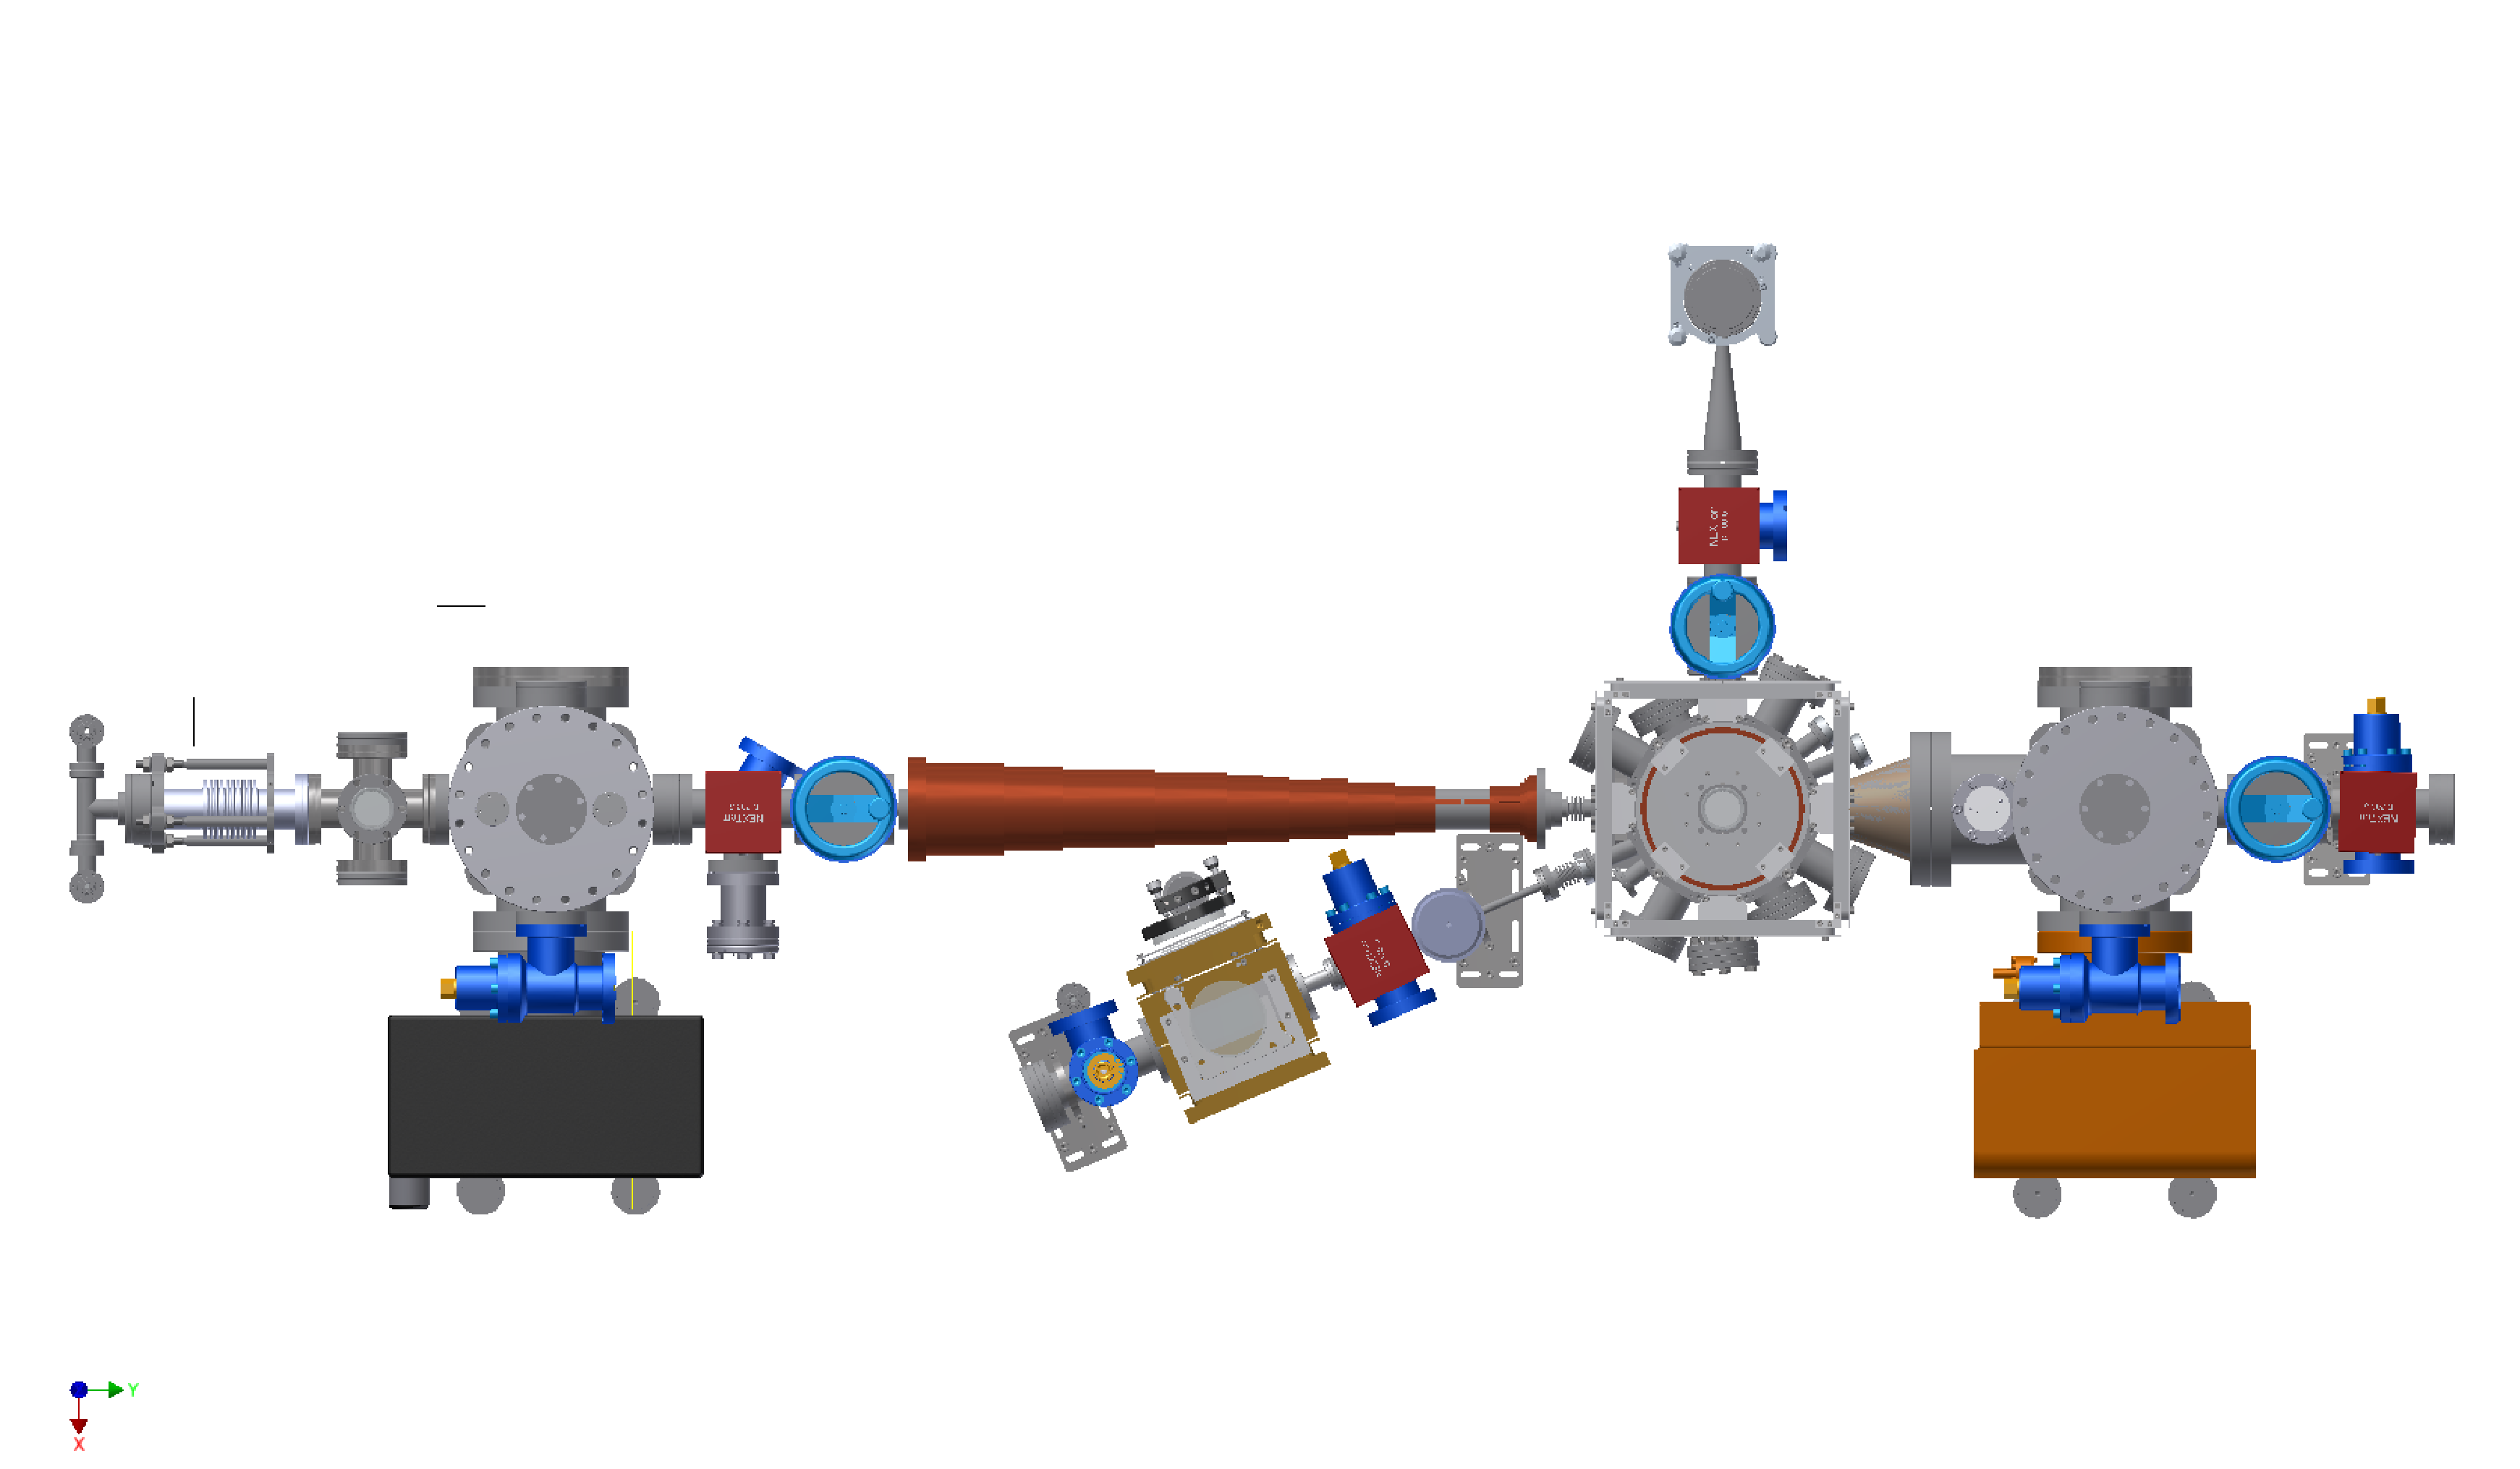
\includegraphics[width=\textwidth]{\figuredir{introduction/apparatus.pdf}}
  \captionsetup{width=.9\textwidth}
  \caption{Apparatus of the cesium experiment. On the left-hand
    side an oven heats up the cesium source. A \gls{2d} \gls{mot} generates a
    particle beam twoards the pipe running through the Zeeman slower in the
    center. The Zeeman slower creates a magnetic field gradient, such that the
    atoms are in resonance with a cooling laser antiparallel to their flight
    direction. In the \gls{3d} \gls{mot} atoms are cooled even further until
    they are transported to a glass cell where they are loaded into the
    optical lattice and the actual experiments are conducted. Thank you to
    Till Klostermann and Hendrik v. Raven for providing the cesium apparatus
    render.}\label{fig:ultracold_atoms_setup}
\end{figure}
The apparatus used for ultracold-atom experiments comprises a vacuum system
with multiple chambers and windows for optical control and manipulation.
\Cref{fig:ultracold_atoms_setup} depicts an exemplary apparatus used
for such an experiment with cesium atoms. The oven on the left-hand side heats
up a cesium source to produce a hos gas of cesium atoms, which will then
diffuse to the right. Two orthogonal pairwise windows enable for transverse
cooling of the atoms in a \gls{2d} \gls{mot}. The Zeeman slower in the center
of the apparatus creates a magnetic field gradient such that the atoms are
always in resonance with a cooling laser antiparallel to the momentum
direction. Through this cooling step many of the atoms can be slowed down in
order to be captured in the \gls{3d} \gls{mot} where the atoms are cooled
further~\cite{Phillips1998}. Finally the atom cloud is transported to a glass
cell at the top, where they are loaded into an optical lattice. The glass
cell is placed between two high numerical aperture objectives for in-situ,
single site imaging and addressing.

One major ingredient to control and manipulate the ultracold atom ensemble in
the experimental chamber is the optical lattice itself. In
\Cref{fig:optical_lattice} a square \gls{2d} optical lattice is illustrated.
\begin{figure}[htb]
  \centering
  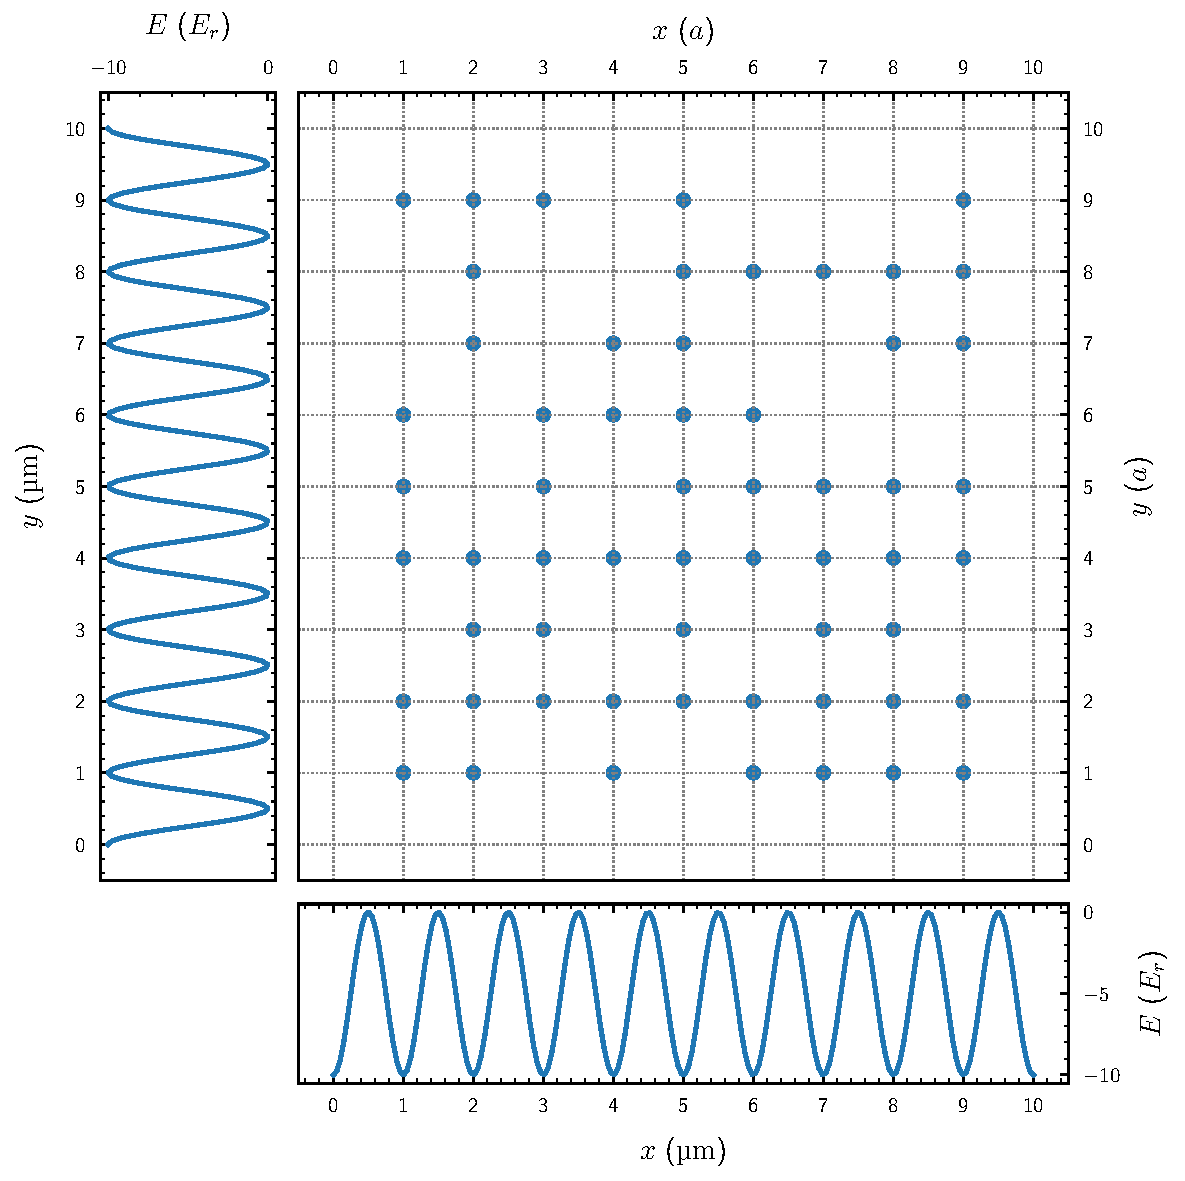
\includegraphics[width=.9\textwidth]
  {\figuredir{introduction/lattice-simple.pdf}}
  \captionsetup{width=.9\textwidth}
  \caption{Simple square \gls{2d} optical lattice. The atoms (blue points) sit
    on their respective lattice site created by the superposition of two
    periodic potentials.
  }\label{fig:optical_lattice}
\end{figure}
The atoms (blue points) sit on their respective lattice sites (nodes in the
gray grid) which are created by the superposition of two orthogonal optical
lattice potentials (outer diagrams)~\cite{Grimm2000}. In such periodic
structures the atomic wave functions already show amazing similarity to the
electron wave functions known from solid states physics but with much higher
energies and longer time scales because of the greater
mass~\cite{Fisher1989,Jaksch1998}. Though the square \gls{2d} optical lattice
already offers many possiblities, one can think of many more variations in
terms of lattice structures like hexagonal lattices or even lattices with a
substructure in the literature known as superlattices. Beside changes to the
global lattice structure we can also think of local changes. In
\Cref{fig:optical_lattice_local_barrier} we show an embodiment of a local
optical lattice used to confine particles.
\begin{figure}[htb]
  \centering
  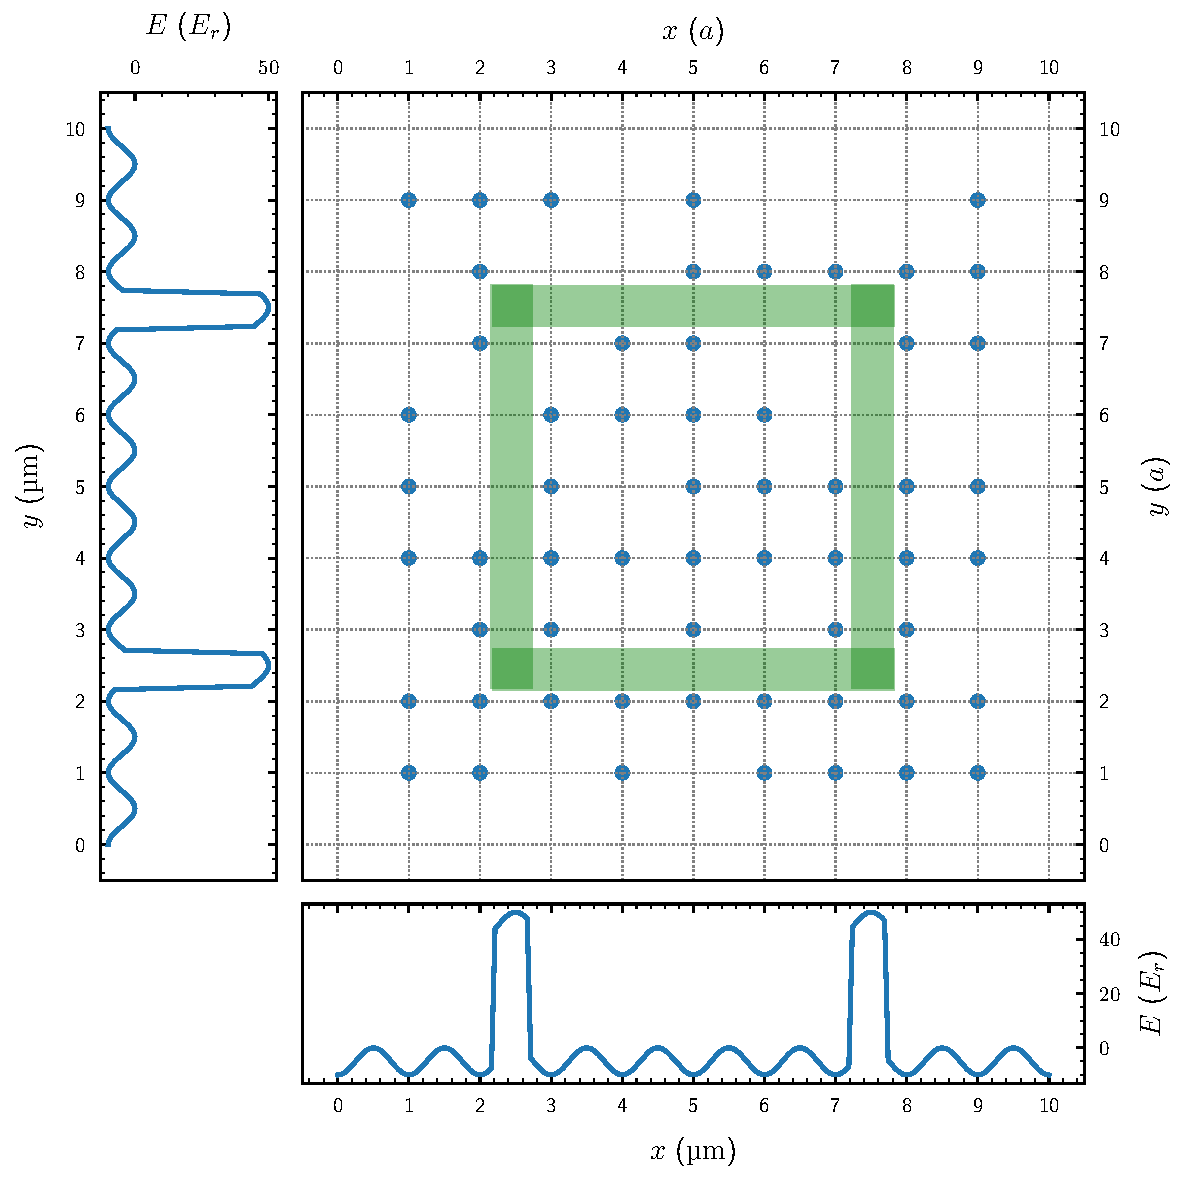
\includegraphics[width=.9\textwidth]
  {\figuredir{introduction/lattice-bar.pdf}}
  \captionsetup{width=.9\textwidth}
  \caption{Simple square \gls{2d} optical lattice with local barrier
    potential. The local barrier potential confines atoms inside the green box
    in a finite homogeneous lattice potential.
  }\label{fig:optical_lattice_local_barrier}
\end{figure}
By changing the barrier height one can control tunel coupling between
neighboring lattice sites which allows one to confine atoms in an optical
lattice without harmonic trap and to study interesting physics at the edges,
i.e.\ topologically protected edge states in the quantum Hall effect, which
cannot be studied without sharp edge heights. A similar potential can be
realized using attractive local potentials to create a potential pot as
illustrated in \Cref{fig:optical_lattice_local_pot}.
\begin{figure}[htb]
  \centering
  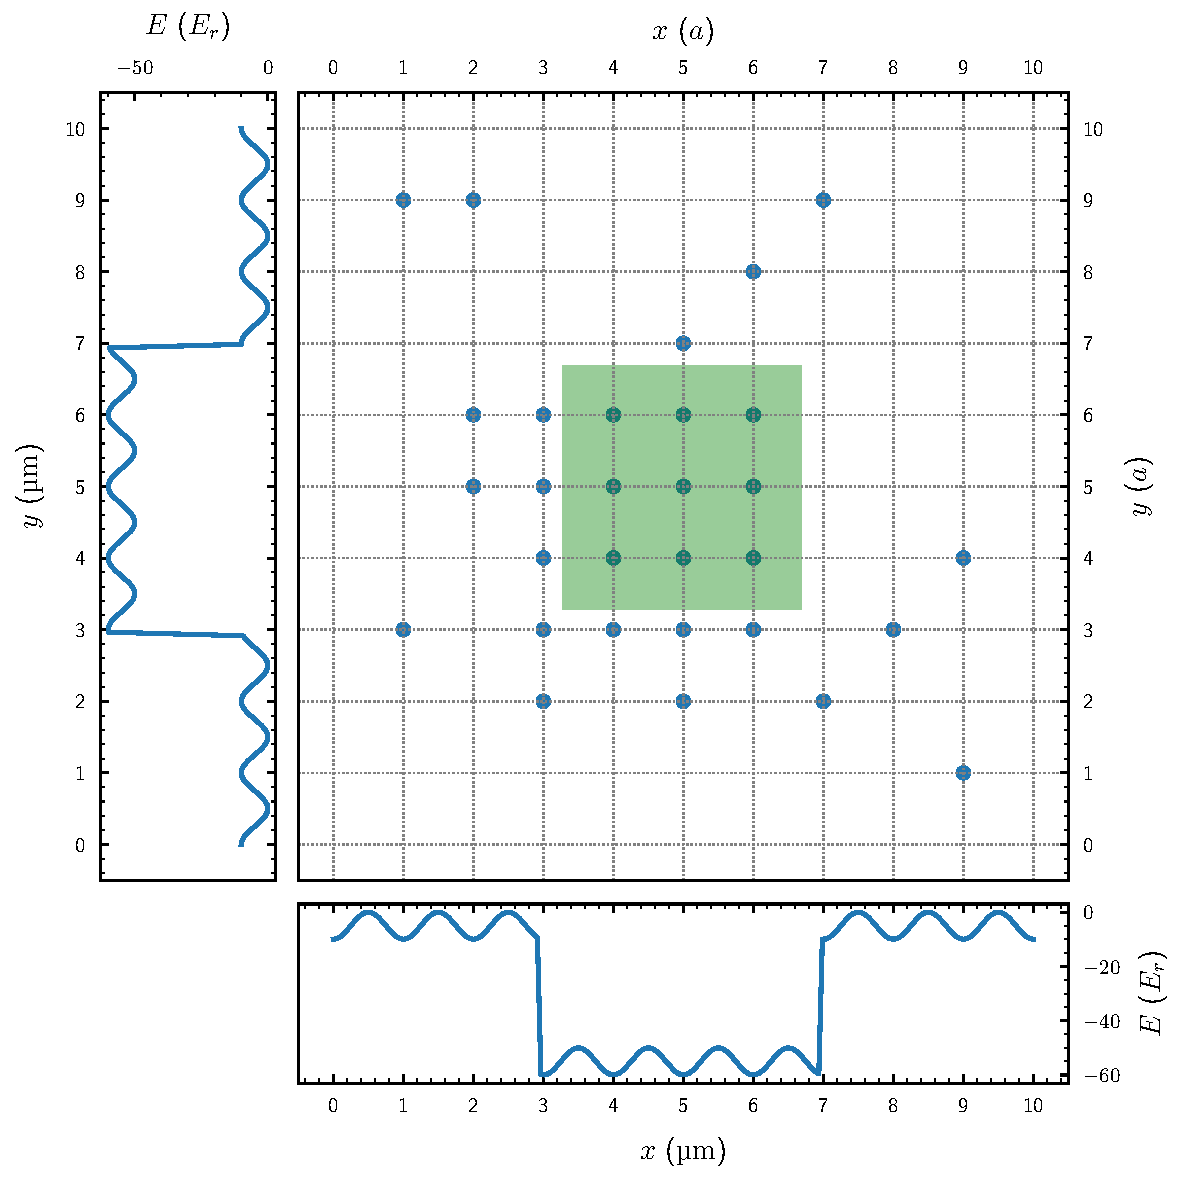
\includegraphics[width=.9\textwidth]
  {\figuredir{introduction/lattice-pot.pdf}}
  \captionsetup{width=.9\textwidth}
  \caption{Simple square \gls{2d} optical lattice with local pot potential.
    The local potental pot draws particles from the unperturbated lattice
    potential to a confined area.
  }\label{fig:optical_lattice_local_pot}
\end{figure}
Dynamically controllable high-resolution potentials could be used, for
instance, to dynamically shape the global potentials to reach lower entropies
or to generate local potentials that affect only a single lattice
site~\cite{Ho2009,Bernier2009,Mazurenko2017}. These are only a few examples,
there are, of course, many more applications of locally controllable optical
potentials.

High-precision local potentials have been created using high-resolution
imaging techniques in combination with digital micromirror devices or spatial
light modulators. The generation of high-quality arbitrary potentials is,
however, challenging and the degree of dynamical control is limited. Another
possibility is the use of arrays of optical tweezers that allow for trapping,
stacking and sorting for particles~\cite{Roxworthy2012}, however, there is no
tunnel coupling between neighboring sites. An alternative approach consists in
the implementation of time-averaged optical potentials. The key concept to
create time-averaged local optical potentials is similar to the operation of
cathode ray tube screens. The idea is to consecutively illuminate a finite
set of points that covers the desired space. A complete passthrough of the
finite set has to occur on a time scale short compared to the time scale
of the observed processes such that on average the passthrough yields an
effective time-averaged potential in the observed process. Yet, only recently,
attempts to interact with local particle clusters through high-precision
time-averaged optical potentials have been reported~\cite{Roy2016}.
In comparison to the state of the art which uses mechanical mirror arrays for
creation of local potentials~\cite{Roy2016} our approach is based on
\gls{aod}. In the following we continue on the ground work laid out in
reference~\cite{Hertlein2017} which provided us with an optical setup for
single-site manipulation using an \gls{aod} as well as the discussion of
aperture limited Gaussian beam propagation.

We will start with the theoretical foundation of optical lattice potentials
and give more details on how the lattice potential is modified under the
presence of an additional perturbation potential. From there on we will
estimate the required time scale set by the hopping frequency and energy bands
of the atoms between neighboring lattice sites. After a short introduction
to direct digital signal synthesis we will calculate, if and how the \gls{dds}
meet the previously determined demands. That in place we can continue with
an overview of our experimental setup and results. The experiments separate in
a two parts: the first one concerns a detailed understanding of the radio
electronics, which powers the \gls{aod} and the second one is dedicated to the
diffraction efficiency of the laser beam after the \gls{aod}, which is
influenced by the \gls{rf} signal and its time-dependence.
